\chapter{Application}\label{chp:4}
As mentioned before, this thesis idea relies on the previously explained methods. Therefore, we performed several applications in the following sections to address and solve the localization problem regarding the autonomous vehicle after studied thoroughly the related works and the theoretical backgrounds. As a first step, we explained the application of every single method. We, next, demonstrated the improvement of them by combining with each other which is the main contribution of this thesis to improve previously mentioned localization techniques.
\par Of note, this chapter was conducted by exploiting remarkable amount of open-software otherwise it would not be possible to make progress without them in given short time span. 

\section{Wheel Odometry}\label{sec:wheel_odometry}
Wheel odometry node\footnote{It can simply be thought an executable file in ROS package} receives the wheel displacement and the steering angle information from sensors to calculate the displacement of the vehicle in a certain time slot. As a consequence, the note delivers pose and velocity information in local frame as well as heading angle and its rate.
\par The odomety algorithm uses the known kinetic equations to generate the outputs as follows:
\\
\begin{align}
  &V_{left} = \Delta X_L*D_n/ \Delta t\\
  &V_{right} = \Delta X_R*D_n/ \Delta t\\
  &V_x = (V_{left}+V_{right})/2\\
  &R = wheelbase/sin(\alpha)\\
  &\phi = V_x * \Delta t / R\\
  &x \leftarrow x+\Delta x, \hspace{5pt} \Delta x = R * sin(\phi)\\
  &y \leftarrow y+\Delta y, \hspace{5pt} \Delta y = -(R-R*cos(\phi))
\end{align}
%\begin{algorithm}[H]
%\SetAlgoLined
%\KwIn{${\Delta X_L, \Delta X_R, \alpha}$}
%\KwOut{${x, y, \theta}$ as $pose_t$}
%{$\Delta t \leftarrow $ length of time sample}\\
%{$V_x = (V_{left}+V_{right})/2$}\\
%  \eIf(straight motion){$\alpha = 0$}{
%   {$dx, dy, d\theta \leftarrow V_x \Delta t, 0, 0 $}\\
%   }(curvature motion){
%   {$R \leftarrow wheelbase/sin(\alpha)$}\\
%   {$\phi \leftarrow V_x \Delta t / R$}\\
%   {$pose \leftarrow$ \Bigg (
%   \begin{tabular}{c c}
%        {$x\leftarrow x+\Delta x,$} &{$\Delta x = R * sin(\phi)$}  \\
%        {$y \leftarrow y+\Delta y,$} &{$\Delta y = -(R-R*cos(\phi))$}\\
%        {$\theta \leftarrow d\theta * \Delta t$}
%   \end{tabular}
%   \Bigg)}
%  }
%  \Return {$pose_t$}
% \caption{Odometry Motion Model}
%\end{algorithm}

\noindent where $V_{left/right}$ are the velocity of left and right wheel respectively, which are calculated over elapsed time $\Delta t$. $\alpha$ is steering angle which is provided by steering wheel for calculating $\phi$ is heading angle and as a last,  position of the vehicle is estimated in direction of $x$ and $y$ in local frame by using turning radius $R$ which depends on steering angle $\alpha$ and difference between front and rear wheel $wheelbase$.
%we can easily derive displacement of the car over time in equation:
\vspace{-0.5cm}
\begin{figure}[H]
\centering
\subfloat[Wheel and steering wheel based odometry ]{\boxed{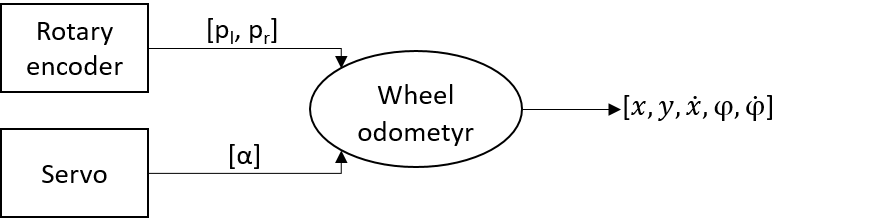
\includegraphics[height=2cm,width=6cm]{odom_node}}\label{fig:odom_pose}}
\hspace{30pt}
\subfloat[Wheel and IMU based odometry]{\boxed{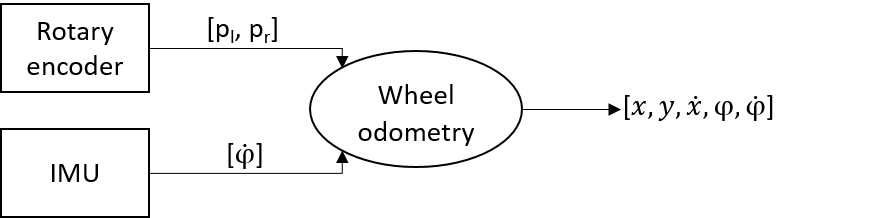
\includegraphics[height=2cm,width=6cm]{odom_node_imu}}\label{fig:odom_pose_imu}}
\caption{Wheel Odometry Node}
\label{fig:odometry}
\end{figure}
\vspace{-0.5cm}
\par Please note that, it is assumed that there is no movement w.r.t roll, pitch angle and z-direction. In addition to this, the velocity component in direction of y is "0" since the vehicle unable to catch any lateral force. Also, it calculates odometry in two different ways as shown in Figure \ref{fig:odometry}. Figure \ref{fig:odom_pose}, it calculated the vehicle heading angle and rate by using steering angle. Figure \ref{fig:odom_pose_imu}, IMU was used to get directly these two values without performing any mathematical effort. The results of these two approaches are presented in the following section.

\section{Extended Kalman Filter (EKF)}
In this section, our task was to fuse data of IMU and odometry data. As already mentioned in the previous chapter, EKF\footnote{\url{http://wiki.ros.org/robot_localization}} from ROS library was used into this thesis. Therefore, we have to only decide that which state we would like to estimate and what are our observation data from sensors. To proceed with EKF, we first introduce what state we can estimate and how we configure them in state estimation node \cite{kalman7}. In this node, the vehicle can be track in 15 different dimension like position, velocity and acceleration in 3D Cartesian coordinate system and in Euler angles as well as their rates and it shows as configuration matrix as follow:
\begin{equation*}\label{eq:state}
 \begin{bmatrix}
X & Y &Z\\
roll& pitch& yaw&\\
\dot X & \dot Y& \dot Z\\
\dot {roll} & \dot {pitch}& \dot {yaw}\\
\ddot X & \ddot Y& \ddot Z
\end{bmatrix}   
\end{equation*}
\par In configuration phase, we should decide which parameter should be fused. As shown in figure \ref{fig:odometry}, the odometry node provides x, y position in the local reference frame, velocity and heading rate in the body frame, while IMU provides heading rates and linear acceleration in body frame w.r.t roll, pitch, yaw and x, y, z respectively.
\begin{figure}[H]
    \centering
    \boxed{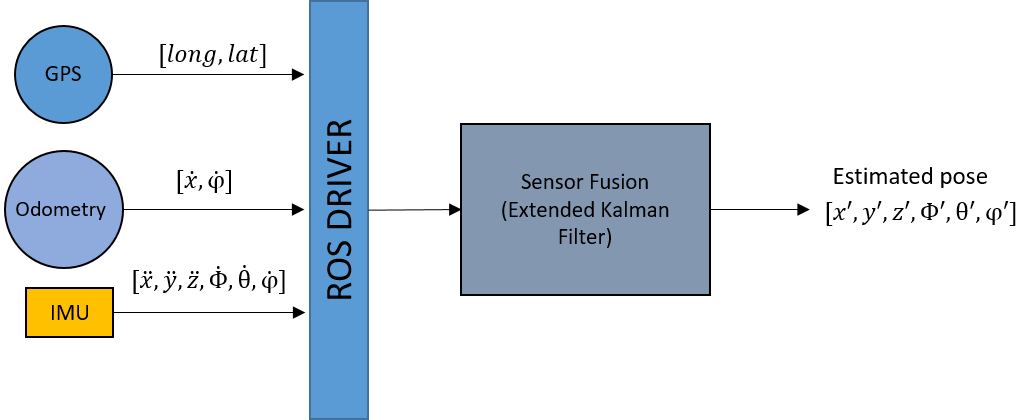
\includegraphics[scale=0.6]{ekf.png}}
    \caption{Data fusion by using EKF}
    \label{fig:ekf_node}
\end{figure}
We fuse the velocity and heading rate provided by odometry node along IMU data into state estimate node. It is important to note that, we do not fuse x, y parameter of odometry as long as IMU exist on the system. The reason is only avoiding to duplicate information since the velocity and absolute position of the vehicle calculated from the same source that may cause the filter to diverge from the desired value. You may also wonder why do we fuse the y component of the velocity ($\dot Y$), in spite of being mentioned as "0" at beginning of this chapter. At first glance, it does not make sense but it actually helps the filter to infer that there is no movement in the y-direction. At the end we have configuration matrix for every single sensor as follows:
\\
\begin{equation*}\label{eq:config}
    \begin{bmatrix}
    false,&false,&false\\
    false,&false,&false\\
    true,&true,&false\\
    false,&false,&true\\
    false,&false,&false
    \end{bmatrix}
\end{equation*}
\\
\noindent where \textbf{\textit{false}} means the value will not be fused while \textbf{\textit{true}} means the value will be fused.

\par As a next and last step, we should tune the process and measurement noise co-variance matrices \textbf {Q} and \textbf{R},respectively. These two matrices are 15 by 15 size, diagonal and all its elements regard to state matrix. Here, there is the rule that we should follow for setting \textbf {Q} and \textbf{R}: Assume that we would like to tune EKF for one measuring parameter, so we have to change the value of the diagonal variable that corresponds to be fused parameter in Q and R matrix. Thus, we can influence the filter in a way that changes its fast to converge true value. For instance, if one can set the diagonal value of R matrix for velocity ($\dot X$) bigger than that measurement’s co-variance so, it makes the filter converge faster. On the other hand, if one can increase the diagonal value of Q matrix and hence it causes the error to grow faster in the state estimate part. Therefore, it effect filter converge faster in principle. However, it is very hard to tune both Q and R matrices but one can reach very optimal result by tuning them. In chapter \ref{chp:5}, it shows the effect of R and Q on EKF.

\section{Normal Distribution Transform (NDT)}
In this section, we describe how NDT method was applied in order to estimate pose in 6 \acrfull{dof}. This application was improved by using \acrfull{pcl}\footnote{\url{http://pointclouds.org/documentation/tutorials/normal_distributions_transform.php}} and Autoware\footnote{\url{https://github.com/CPFL/Autoware}} which are both open source libraries. The basic NDT algorithm is designed to use only point clouds information for finding  most likelihood transformation between the reference and target model as shown in figure \ref{fig:ndt}.
\vspace{-0.5cm}
\begin{figure}[H]
    \centering
    \subfloat[basic NDT]{\boxed{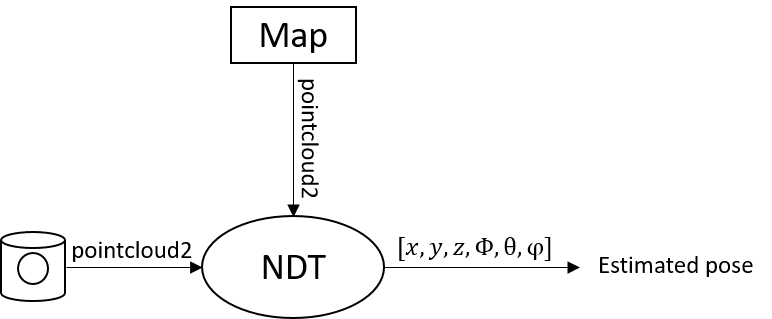
\includegraphics[height=3.5cm,width=7cm]{ndt}\label{fig:ndt}}}
    \hfill
    \subfloat[NDT with wheel odometry]{\boxed{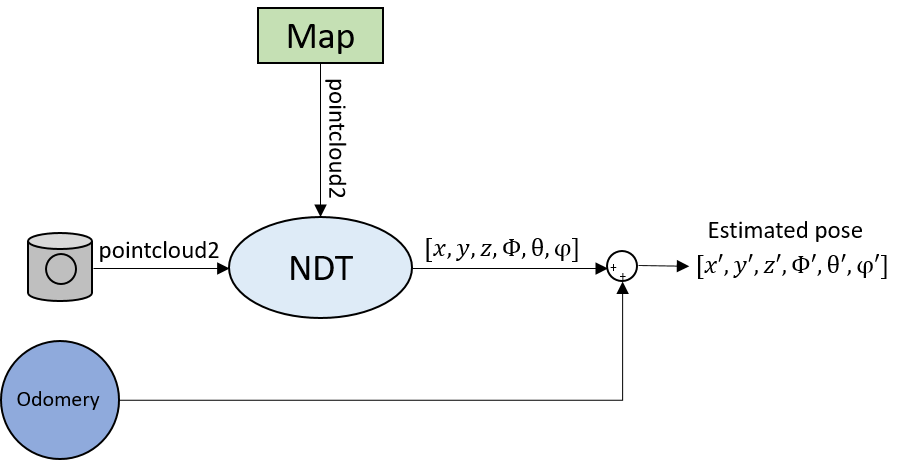
\includegraphics[height=3.5cm,width=7cm]{ndt_odom}}\label{fig:ndt_odom}}
    \caption{Work flow of NDT}
\end{figure} 

\par\noindent NDT tries to extract the position of the vehicle on the prior map. However, the basic NDT has a tendency to lose track of position against any disturbance for example, change of environment conditions. Therefore, we first link the odometry reading with NDT in order to support for tracking pose. Of note, we are not using the position of odometry since it is not only prone to drift but also it uses different frame than NDT. Due to the fact, only the linear and angular velocity of odometry is used to recalculate the relative position. After that, the found position is added to the current position for correcting the estimated position of NDT. Subsequently, NDT node is redesigned as shown in figure \ref{fig:ndt_odom}.

\par However, a further improvement of NDT is needed since odometry has lack of information about the movement of vehicle and it is unreliable for long-term localization as we discussed in section \ref{sec:odom}. At this point, EKF is brought into play to support the algorithm in order to make NDT more robust. We, next, employed EKF with odometry, GPS and IMU data to add NDT as shown in figure \ref{fig:ndt_ekf}. The advantage of employing EKF in this fashion is improving the result and reducing the noise from sensors.
%\par Yet there is another derivation of this application- In this instance, we use two EKF. One is used in the same way as the previous one. The other one is used for fusing NDT, IMU, and odometry as shown in figure \ref{fig:ndt_2ekf}. The purpose of doing this is eliminating unwanted movement of NDT since it estimates the pose of the vehicle in map frame hence it generates discrete jumps in a time period even though it eliminates drift \cite{rep105}. 
%\begin{figure}[H]
%    \centering
%    \setlength{\fboxsep}{0pt}%
%    \setlength{\fboxrule}{1pt}%
%    \fbox{
%    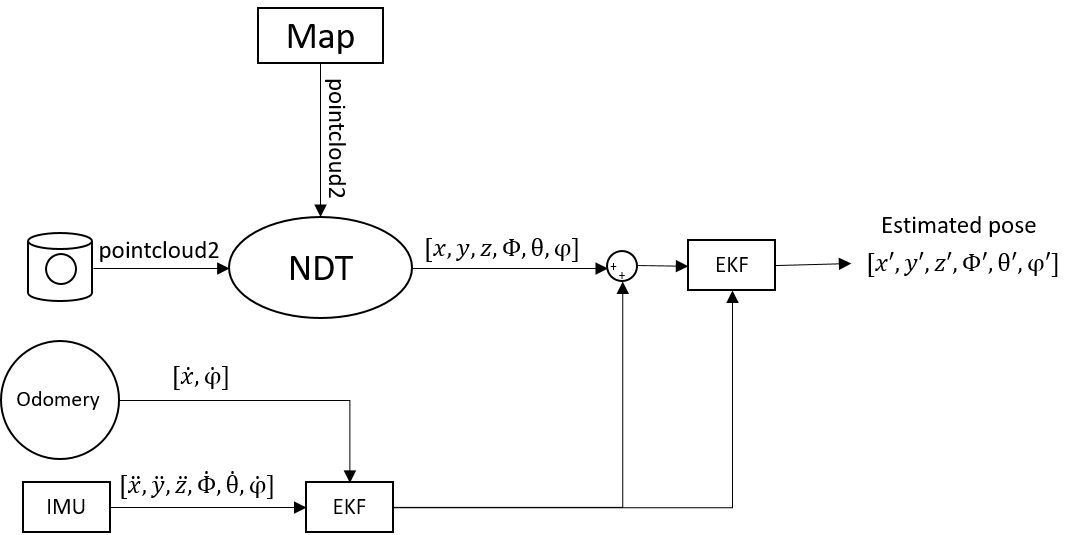
\includegraphics[scale=0.52]{ndt_2ekf}}
%    \caption{Caption}
%    \label{fig:ndt_2ekf}
%\end{figure}
\par On the other hand, the algorithm is yet not capable of self-initialization. As mentioned in section \ref{sec:summary}, NDT and ICP cannot find the matches between two scans unless they do know where to start. Therefore, we had to provide an initial transform between the vehicle and the map. Thus, we approached this problem from GPS perspective. First, we provided static transformation between map and local coordinate by converting the first GPS output longitude and latitude, where a map was started to build, to \acrfull{utm} coordinate by using geodetic tool \cite{utm}. Then, we obtained transformations which are from GPS to map $_{G}^{M}T$ and GPS to vehicle $_{G}^{V}T$. Following this, to find the transformation between map and vehicle $_{V}^{M}T$ we used chain rule property as follows \cite{robotic}:
\begin{align}
    _{G}^{M}T &= _{G}^{V}T \cdot _{V}^{M}T\\
    _{V}^{M}T &= _{V}^{G}T^{-1} \cdot _{G}^{M}T
\end{align}
It should be noted that the heading angle of the vehicle was provided from IMU to find transformation $_{V}^{M}T$ since GPS provides only longitude and latitude information.
\par As a result of these improvements, NDT was transformed into a more robust algorithm than basic NDT as shown in figure \ref{fig:ndt_son}. Hence, NDT becomes more versatile to answer "where am I" and "where am I going" fundamental questions for robot navigation. 
\vspace{-0,5cm}
\begin{figure}[H]
    \centering
    \subfloat[First evolution of NDT by EKF]{\boxed{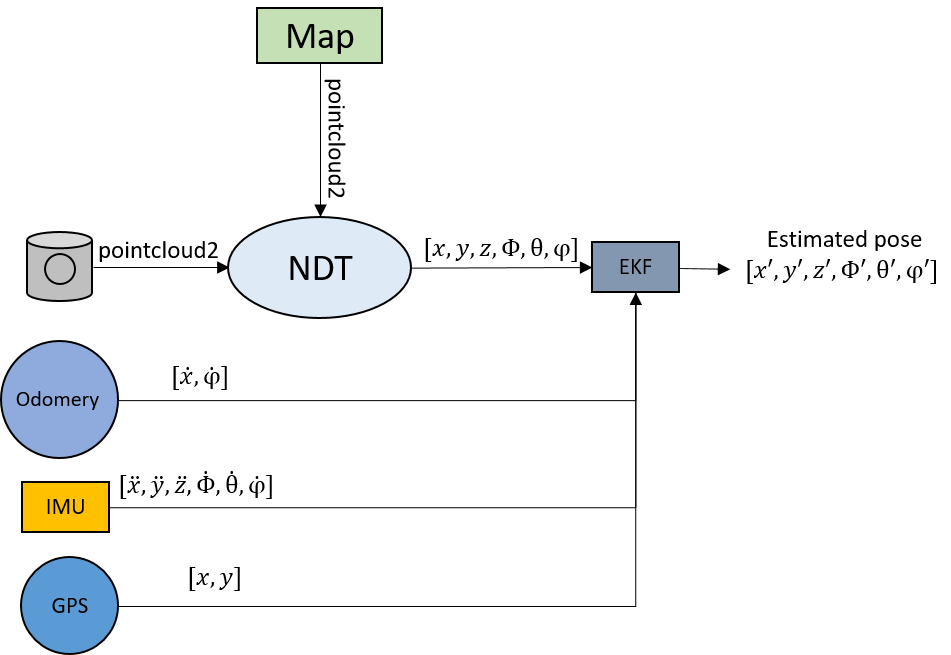
\includegraphics[height=3.5cm,width=7cm]{ndt_ekf}} \label{fig:ndt_ekf}}
    \hfill
    \subfloat[Second evolution of NDT by GPS]{\boxed{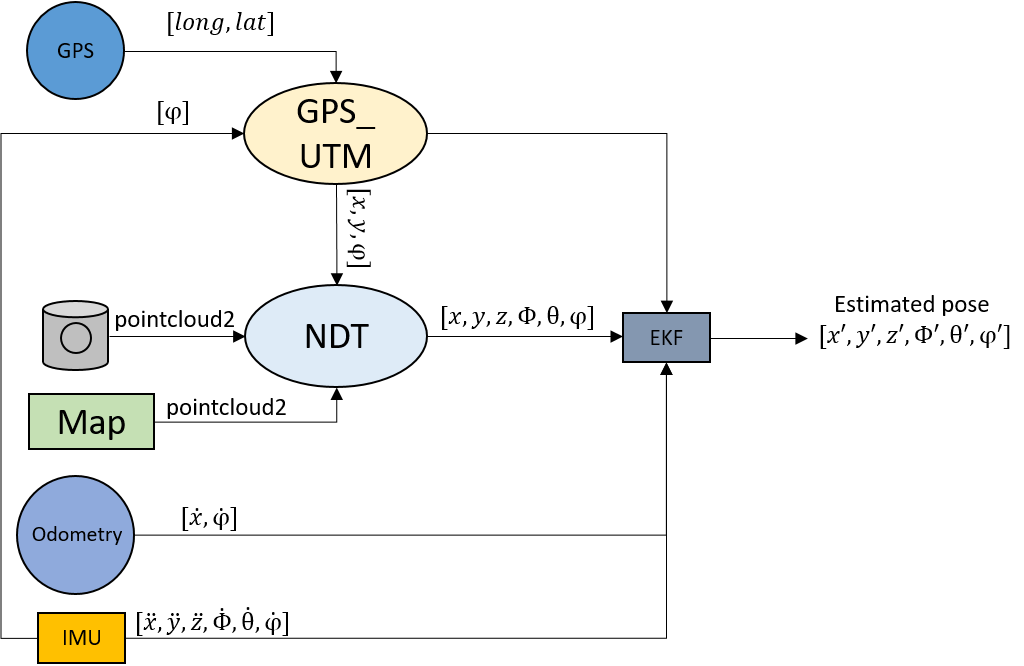
\includegraphics[height=3.5cm,width=7cm]{ndt_son}}\label{fig:ndt_son}}
    \caption{Evolution phase of NDT}
\end{figure}

\section{Iterative Closest Point (ICP)}
To estimate the position of the vehicle upon point scan data, ICP is commonly used over two decades and this section describes ICP that addressed the localization problem. ICP algorithm is treated in the same fashion as NDT in this section. In theory, ICP by itself should provide result that are more accurate since, ICP uses every single point in two scans for finding the most plausible transformation  as long as initial transformation is known as shown in figure \ref{fig:icp}. 
\vspace{-0.5cm}
\begin{figure}[H]
  \centering
  \subfloat[Illustration of ICP Matching \textbf{Source}: Tudor Paun \cite{icp5}]{\boxed{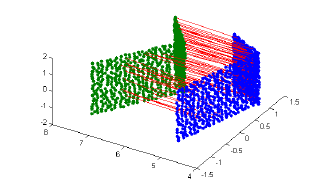
\includegraphics[height=3.5cm,width=7cm]{icp}}\label{fig:icp}}
  \hfill
  \subfloat[Work flow of ICP]{\boxed{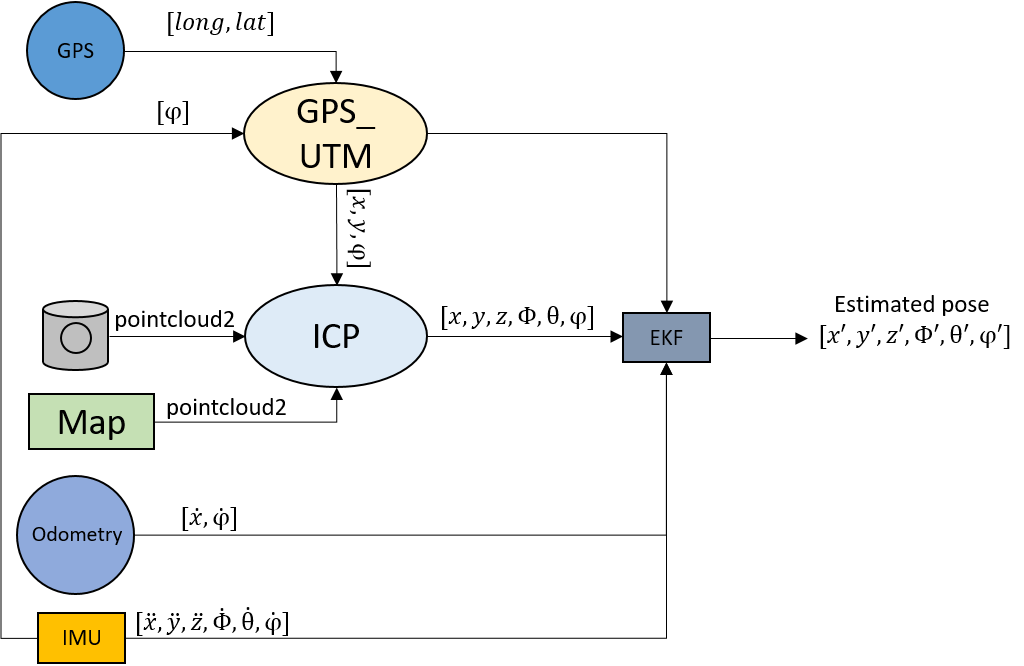
\includegraphics[height=3.5cm,width=7cm]{icp_son}}\label{fig:icp_son}}
    \caption{ICP}
\end{figure}
To provide the initial position to ICP, we did some improvement which was stated shortly as follows:
\begin{itemize}
    \item Integrating odometry to ICP
    \item Integrating EKF to ICP
    \item Integrating GPS to ICP
\end{itemize}
and see figure \ref{fig:icp_son} for the improved ICP.

\section{Summary}
The aim of this chapter is having one localization algorithm that provides redundancy. It can be thought of taking a back-up of the system or preventing any discontinuity on a running system even if any failure happened on the subsystem. In other words, the system must be capable to mitigate/eliminate against any failure on the system by using or swapping all available sources.%todo:add
\par Considering the fact that, we presented the four different localization methods which deal with the localization problems in a different ways. First, we applied odometry which relies on dead reckoning. Although, odometry is one of the main sources of robot navigation, as stated  in Javier Hidalgo Carrió's study \cite{odomja}, pose estimate by using odometry generally accumulates errors over time.To overcome this problem, we need to use additional sensory information. Therefore, we employed EKF and explained how to configure EKF in a way that fusing different sensors. Following that, we first applied two scan registration method in basic level which are NDT and ICP. These two methods are commonly used in different SLAM algorithms as mentioned in \cite{6D_SLAM}, \cite{NDT_SLAM} and we showed their evolution phases by combining odometry, GPS, IMU with EKF methods.


